\documentclass[12pt,a4paper,hyperlinks]{rapport_unif}
\usepackage[utf8]{inputenc}
\usepackage{pdfpages}
\usepackage{tabularx}
\usepackage{booktabs}
\usepackage{parskip}
\usepackage{listings}
%\usepackage{color}
%
%\definecolor{dkgreen}{rgb}{0,0.6,0}
%\definecolor{gray}{rgb}{0.5,0.5,0.5}
%\definecolor{mauve}{rgb}{0.58,0,0.82}
%
%\lstset{frame=tb,
%  language=VHDL,
%  aboveskip=3mm,
%  belowskip=3mm,
%  showstringspaces=false,
%  columns=flexible,
%  basicstyle={\small\ttfamily},
%  numbers=none,
%  numberstyle=\tiny\color{gray},
%  keywordstyle=\color{blue},
%  commentstyle=\color{dkgreen},
%  stringstyle=\color{mauve},
%  breaklines=true,
%  breakatwhitespace=true,
%  tabsize=3
%}
\usepackage[squaren, Gray, cdot]{SIunits}
\usepackage{amsmath}
\usepackage[tableposition=top]{caption}
\captionsetup[table]{singlelinecheck=off}
\renewcommand{\arraystretch}{1.2}
\usepackage{microtype}
\usepackage{cleveref}

\defStudentTwo[Cauz]{Marine}
\defStudentTwoNumber{s111246}
\defStudentTwoMail{marine.cauz@student.ulg.ac.be}
\defStudentTwoYear{1st master Electrical Engineering}

\defStudentThree[Di Carlo]{Gr\'egory}
\defStudentThreeNumber{s102543}
\defStudentThreeMail{gregory.dicarlo@student.ulg.ac.be}
\defStudentThreeYear{1st master Electrical Engineering}

\defStudentFour[Woszczyk]{Hubert}
\defStudentFourNumber{s104163}
\defStudentFourMail{hwoszczyk@student.ulg.ac.be}
\defStudentFourYear{1st master Electrical Engineering}

\author{Marine Cauz & Florent Bourghelle & Gregory Di Carlo & Hubert Woszczyk}
\cours{ELEN0037 - Microelectronics and IC design}
\title{Lab 1 Report}
\date{22/03/2015}

\lhead{}
\chead{}

\begin{document}
\lstset{language=VHDL}
\maketitle
\newpage
\section{Theoretical considerations}
\subsection{Available resources}
The chip on-board of the de0-nano is the EP4CE22F19C6N. It is composed of 22,320 logic elements, 594kbits of embedded memory and has 112 available GPIO.

The de0-nano development board provides access to 72 I/O pins, 5V and 3.3V power pins. Additionally to the embedded memory, there are 32mB of SDRAM and 2kB of I2C EEPROM available.

\section{Displaying a red rectangle onscreen}
\subsection{Code}
The program is a bare-bone vga controller that displays a red rectangle in the middle of a screen. The circuit is modelled as an entity \emph{vga} that generates vertical and horizontal synchronization signals and the green, blue and red color signals. A 50MHz oscillator drives this entity, as the sole input.

The synchronization signals are active low and signal the end of lines and frames. The red, green and blue signals define the color of the pixel that is currently being sent over the port.

\section{Creation, simulation and programming of a project}
\subsection{Simulation}
The results are exactly what was expected. The vertical synchronization occurs much less frequently(once per frame) than the horizontal one(once per line). 

\Cref{fig:sim1} shows that relationship between lines and frames. The vertical synchronization signal is on top, the horizontal synchronization signal is in the middle and the red signal is at the bottom. A zoom on the signals is shown on \cref{fig:sim2}.

On both figures, the red rectangle is clearly present, as a series of pulses that occur exactly between two horizontal synchronizations. The series itself occurs between 2 vertical synchronizations. 

\begin{figure}[htp]
\centering
	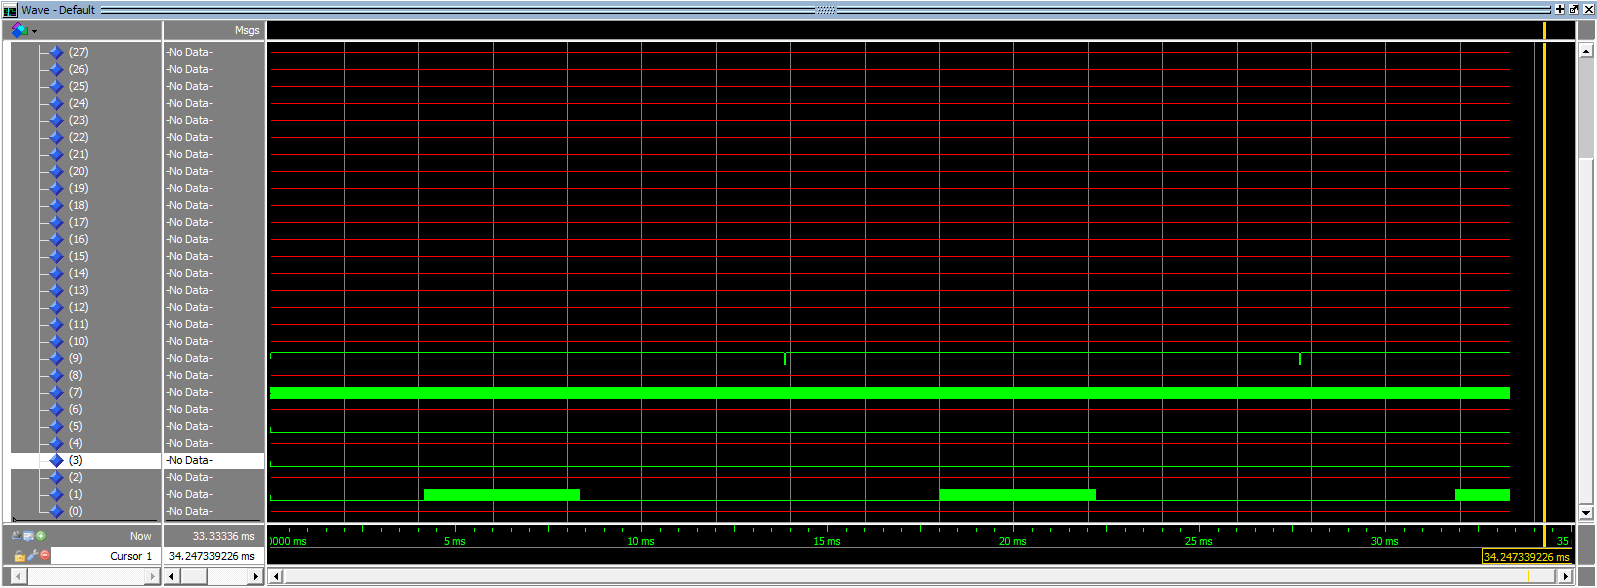
\includegraphics[width=0.9\textwidth]{figures/simu1}
	\caption{RTL Simulation - The vertical synchronization is clearly less frequent than the horizontal one, as it should. The red rectangle is also visible, as the signal on the bottom.}
	\label{fig:sim1}
\end{figure}

\begin{figure}[htp]
\centering
	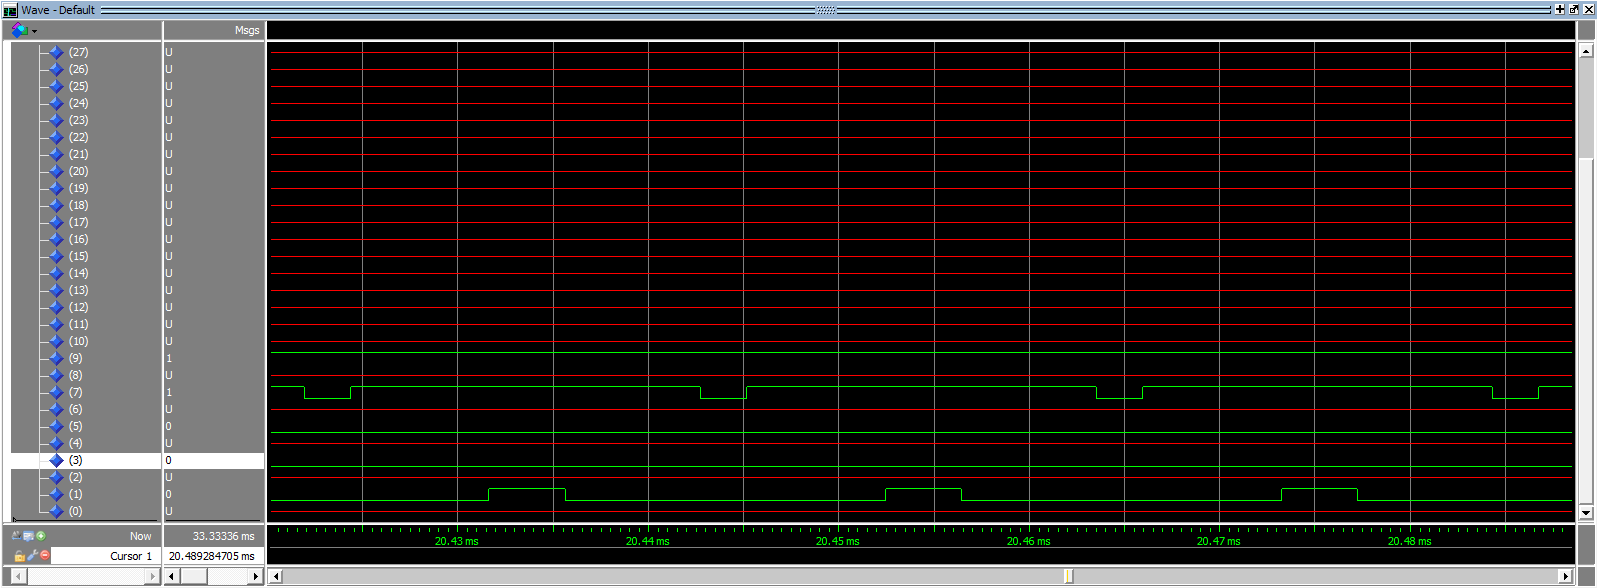
\includegraphics[width=0.9\textwidth]{figures/simu2}
	\caption{RTL Simulation - Zoom on 3 lines, with their delimiting horizontal synchronization signals clearly shown. The red rectangle is once more easily identified as the signal on the bottom.}
	\label{fig:sim2}
\end{figure}

\subsection{Warnings}
\begin{itemize}
\item \emph{10873 Using initial value X (don't care) for net "signal"} : this warning tells us we didn't specify a default value for some of the output pins.
\item \emph{13024 Output pins are stuck at VCC or GND} : some output pins do not change their value throughout the program. Quartus implies this output is potentially useless.
\end{itemize}

\subsection{RTL Netlist viewer}
The active (Red, green, blue, hsync, vsync) output ports of the \emph{vga} entity get a register. In addition, each of the signals defined as part of the architecture gets a register too.

When locating the line that spawned a register, Quartus shows the line that declares the signal or output port. So, for example, the register  \emph{blue\_signal} corresponds to the following line

\begin{lstlisting}
29  signal blue_signal : std_logic;
\end{lstlisting}

%All signals declared in the architecture of the \emph{vga} entity get a register. In particular, the following lines correspond to registers :
%\begin{enumerate}
%\item register h\_cnt refers to the line that instantiates a register h\_cnt
%\item register v\_cnt refers to the line that instantiates a signal v\_cnt
%\item register vertical\_en refers to the line that instantiates a signal vertical\_en
%\item register horizontal\_en refers to the line that instantiates a signal horizontal\_en
%\item red green and blue signals
%\item GPIO\_1\_D(1,3,5,7,9)
%\end{enumerate}

\subsection{Pin planner}
The connector is connected to the GPIO-1 header, but we still have to specify where the signals have to be outputted from the FPGA. That is done in \cref{table:pins}. 

\begin{table}[htp]
\centering
\caption{Pin attribution of output signals}
\begin{tabularx}{\textwidth}{@{}X X X@{}}
\toprule
Signal & GPIO & FPGA pin\\
\midrule
Red & GPIO\_11 & PIN\_T15 \\
Green & GPIO\_13 & PIN\_T13 \\
Blue & GPIO\_15 & PIN\_T12 \\
$h_{syn}$ & GPIO\_17 & PIN\_T11 \\
$v_{sync}$ & GPIO\_19 & PIN\_R11 \\
Ground & GPIO\_1 & - \\
Clock & - & PIN\_R8 \\
\bottomrule
\end{tabularx}
\label{table:pins}
\end{table}

The clock is assigned to pin R\_8 because the devboard includes a 50MHz oscillator directly connected to this pin.

%Observez tous les rapports qui vous sont soumis. A quoi servent-ils ? Que sont les différents modèles? Essayez avec différentes valeurs d’horloge et de délais de sortie minimum et maximum. Que se passe-t-il ? Écrivez vos constatations de manière détaillée, et expliquez le fonctionnement des analyses de timings ainsi que les résultats qui peuvent être déduits. Aussi, regardez l’effet des contraintes de timings sur le Fitter. Que se passe-t-il ?
\subsection{Timings}
These report help us build circuits that behave coherently at given frequencies. Some reports tell us how much slack each signal gets given the propagation delays in fast or slow silicon. Based on these slacks, TimeQuest gives some frequency range in which our circuit could operate.

There are 3 models :
\begin{itemize}
\item Slow 1200mV 0C models the timing of the signals in a slow silicon at 0C.
\item Slow 1200mV 85C models the timing of the signals in a slow silicon at 85C, which is considered to be the higher end of operating temperature.
\item Fast 1200mV 0C models the timing of the signals in a fast silicon at 0C. That can be considered as the best case.
\end{itemize}

When setting the max delay on the clock transition to 17ns the timing analysis fails, because several signals can't get updated before the next clock transition. 

First, \emph{Slow 1200mV 85C Model} requires a maximum frequency of $45.9 MHz$ but after our modifications we work with a $50MHz$ frequency. The setup slack is negative for 3 signals. The first signal is between $GPIO\_1\_D[1]~reg0$ and $GPIO\_1\_D[1]$. The second one is between $GPIO\_1\_D[7]~reg0$ and $GPIO\_1\_D[7]$ and the last one between $GPIO\_1\_D[9]~reg0$ and $GPIO\_1\_D[9]$. These 3 negative slacks come from the fact that the data is stable during a time lower than the required setup time before a rising edge of the clock. Indeed, we impose a maximal output delay of 17ns with a period of rising edges every 20 ns.

Then, the second model is \emph{Slow 1200mV 0C Model}. For this model the maximum frequency is $47MHz$ and so when we work at $50MHz$ we have also a problem because the output is not updated before the next period of clock. Again, the setup time is to blame and with the sames 3 signals.

The last model, the \emph{Fast 1200mV 85C Model} works with the constraints imposed. In this case the setup and hold slack are both positive.

\subsection{Exercise}
The following code allows us to display a color changing  central square. We only had to add a counter, to count the elapsed time, and a new signal to represent the current color of the square.

\subsection*{vga\_colors.vhd :}
\begin{lstlisting}
library ieee;
use ieee.std_logic_1164.all;
use ieee.std_logic_arith.all;
use ieee.std_logic_unsigned.all;

entity vga_colors is
Port(
	CLOCK_50		: in std_logic;
	GPIO_1_D		: out std_logic_vector(33 downto 0)	
	);
end entity vga_colors;

architecture vga_arch_colors of vga_colors is	-- Sync signal
	signal h_sync			: std_logic;
	signal v_sync			: std_logic;
	-- Video Enables
	signal video_en		: std_logic;
	signal horizontal_en	: std_logic;
	signal vertical_en	: std_logic;
	-- Color signal
	signal red_signal		: std_logic;
	signal green_signal	: std_logic;
	signal blue_signal	: std_logic;
	-- Sync Counters
	signal h_cnt : std_logic_vector(10 downto 0) := (others => '0');
	signal v_cnt : std_logic_vector(10 downto 0) := (others => '0');
	-- Sync Colors : 
	signal color : std_logic_vector(2 downto 0) := "000";

begin

vga_gen : process

variable time_cnt : integer := 50000000; 

begin
wait until ( (CLOCK_50' event) and (CLOCK_50 = '1') ) ;

time_cnt := time_cnt-1;
if(time_cnt = 0) then
	color <= color + "001";
	time_cnt := 50000000;
end if;

-- Generate Screen
if( v_cnt >= 0) and (v_cnt <= 799) then
	red_signal <= '0';
	green_signal <= '0';
	blue_signal <= '0';
	if( ((v_cnt >= 200) and (v_cnt <= 400)) 
		and ((h_cnt >= 300) and (h_cnt <= 500)) ) then
		case color is 
		when "000" =>
			red_signal <= '0';
			green_signal <= '0';
			blue_signal <= '0';
		when "001" =>
			red_signal <= '1';
			green_signal <= '0';
			blue_signal <= '0';
		when "010" =>
			red_signal <= '0';
			green_signal <= '1';
			blue_signal <= '0';
		when "011" =>
			red_signal <= '0';
			green_signal <= '0';
			blue_signal <= '1';
		when "100" =>
			red_signal <= '1';
			green_signal <= '1';
			blue_signal <= '0';
		when "101" =>
			red_signal <= '0';
			green_signal <= '1';
			blue_signal <= '1';
		when "110" =>
			red_signal <= '1';
			green_signal <= '0';
			blue_signal <= '1';
		when "111" =>
			red_signal <= '1';
			green_signal <= '1';
			blue_signal <= '1';
		end case;

	end if;
end if;

-- Generate Horizontal Sync
if(h_cnt <= 975) and (h_cnt >= 855) then
	h_sync <= '0';
else
	h_sync <= '1';
end if;

-- Reset Horizontal Counter
if(h_cnt = 1039) then
	h_cnt <= "00000000000";
else
	h_cnt <= h_cnt + 1;
end if;

-- Reset Vertical Counter
if (v_cnt >= 665) and (h_cnt >= 1039) then
	v_cnt <= "00000000000";
elsif (h_cnt = 1039) then
	v_cnt <= v_cnt + 1;
end if;

-- Generate Vertival Sync
if (v_cnt <= 642) and (v_cnt >= 636) then
	v_sync <= '0';
else
	v_sync <= '1';
end if;

-- Generate Horizontal Enebale
if(h_cnt <= 799) then
	horizontal_en <= '1';
else
	horizontal_en <= '0';
end if;

-- Generate Vertical Enable
if (v_cnt <= 599) then
	vertical_en <= '1';
else
	vertical_en <= '0';
end if;

video_en <= horizontal_en and vertical_en;

-- Assign physical signal to vga
GPIO_1_D (1) <= red_signal and video_en;
GPIO_1_D (3) <= green_signal and video_en;
GPIO_1_D (5) <= blue_signal and video_en;
GPIO_1_D (7) <= h_sync;
GPIO_1_D (9) <= v_sync;

end process vga_gen;

end architecture vga_arch_colors;
\end{lstlisting}
\section{Project debug}
\subsection{Code analysis}
We were asked to analyse the code of the Gsensor project.
\Cref{fig:diagram} presents the different entities used in this project. We figured out that the code controls 8 LED's on the DE0-nano board according to the orientation of the accelerometer's x-axis.

\begin{figure}[htp]
 \centering
 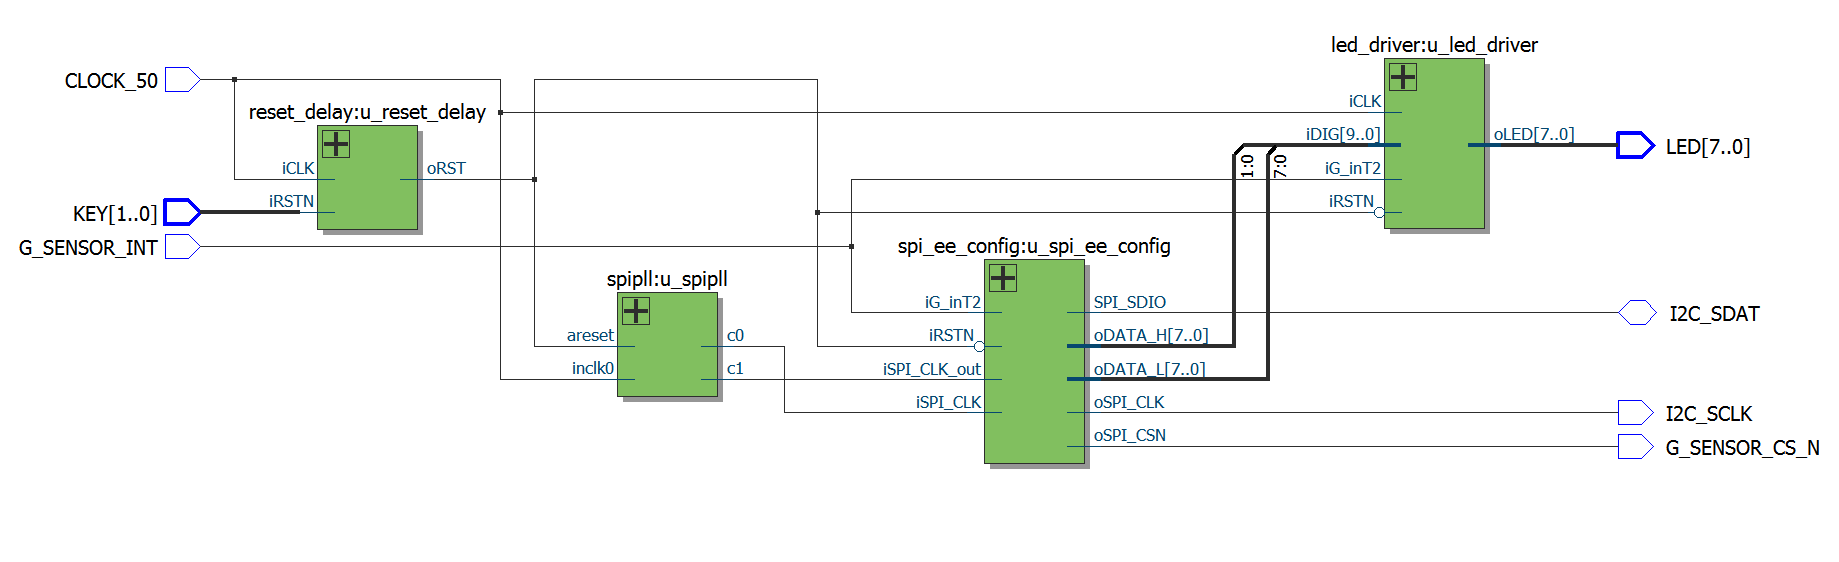
\includegraphics[width = \textwidth]{figures/diagram}
 \caption{Diagram of the different entities - Gsensor project}
 \label{fig:diagram}
\end{figure}

The project contains the following entities:
\begin{itemize}
\item \textit{gsensor} : This is the main entity that gathers and links all the sub-entities and all the internal signals.
\item \textit{reset\_delay} : Allows the reset of all the signals when the \textit{KEY0} button is pushed or at the end of a 20 bits counter.
\item \textit{spipll} : The goal of this entity is to generate a new clock signal (slower than the $50MHz$) which will be used by \textit{spi\_ee\_config} to communicate with the accelerometer.
\item \textit{spi\_ee\_config} : The entity responsible for the communication with the accelerometer. Data are exchanged using the SPI(with 3 wires) protocol. The information about the acceleration of the x-axis (coming from the captor) is stored in signals \textit{oDATA\_L} (low bytes) and \textit{oDATA\_H} (high bytes). Then the measure is sent to the \textit{led\_driver} entity.
\item \textit{led\_driver} : Its job is to interpret the data coming from \textit{spi\_ee\_config} in order to drive the 8 LED's through its output vector of 8 bits.
\end{itemize}

\section{Final exercise}
In order to realize this exercise, we reused the code of the \textit{Gsensor} project explained previously. We first replaced the entity \textit{led\_driver} by our entity \textit{vga}. So, we had to create the mapping between the signals of \textit{vga} and the signals coming from the other entities (see file \textit{gsensor.vhd} below). We also had to modify the file \textit{spi\_ee\_config} so that the fpga can retrieve the data about the acceleration of the y-axis from the accelerometer. The last thing left to do is to modify the \textit{vga.vhd} file in such a way that the position of the square is determined by the orientation of the DE0-nano board. So, the entity \textit{vga} has to take into account the data coming from the accelerometer to position the coloured square at the right place on the screen.

Here is the code of the 3 modified entities :
\subsection*{gsensor.vhd :}
\begin{lstlisting}
----------------------------------------------
-- gsensor.vhd
-- sindredit@gmail.com 16 Feb 2012
-- Top level design
----------------------------------------------

-- Library importation
LIBRARY IEEE;
USE IEEE.std_logic_1164.all;

-- Entity declaration
entity gsensor is
    -- Port ----------------------------------
    -- Comes from other files or from the card
    port (
	CLOCK_50	: IN std_logic;
	KEY		: IN std_logic_vector(1 DOWNTO 0);   
	G_SENSOR_INT	: IN std_logic;   -- G_Sensor Interrupt PIN_M2
		
	I2C_SDAT	: INOUT std_logic; -- EEPROM data PIN_F1
	I2C_SCLK	: OUT std_logic;  -- EEPROM clock PIN_F2
	G_SENSOR_CS_N	: OUT std_logic;   -- G_Sensor chip select PIN_G5
      
	out_red		: out std_logic;
	out_green	: out std_logic;
	out_blue	: out std_logic;
	out_h_sync	: out std_logic;
	out_v_sync	: out std_logic
	);
end entity;
    
-- Architecture ------------------------------------------------------	
-- This file only
architecture synth of gsensor is

   --=======================================================
   --  REG/WIRE declarations
   --=======================================================
   SIGNAL dly_rst                  :  std_logic;   
   SIGNAL spi_clk                  :  std_logic;   
   SIGNAL spi_clk_out              :  std_logic;   
   SIGNAL data_x                   :  std_logic_vector(15 DOWNTO 0);
   SIGNAL data_y                   :  std_logic_vector(15 DOWNTO 0);
   
   SIGNAL G_SENSOR_CS_N_xhdl2      :  std_logic;   
   SIGNAL I2C_SCLK_xhdl3           :  std_logic;   

BEGIN
   --LED <= LED_xhdl1;
   G_SENSOR_CS_N <= G_SENSOR_CS_N_xhdl2;
   I2C_SCLK <= I2C_SCLK_xhdl3;
	
   -- u_reset_delay
   u_reset_delay : entity work.reset_delay 
      PORT MAP (
         iRSTN => KEY(0),
         iCLK => CLOCK_50,
         oRST => dly_rst);   
   
   -- u_spiipll
   u_spipll : entity work.spipll 
      PORT MAP (
         areset => dly_rst,
         inclk0 => CLOCK_50,
         c0 => spi_clk,
         c1 => spi_clk_out);   
   
   -- u_spi_ee_config
   u_spi_ee_config : entity work.spi_ee_config 
      PORT MAP (
         iRSTN => NOT dly_rst,
         iSPI_CLK => spi_clk,
         iSPI_CLK_OUT => spi_clk_out,
         iG_INT2 => G_SENSOR_INT,
         oDATA_XL => data_x(7 DOWNTO 0),
         oDATA_XH => data_x(15 DOWNTO 8),
			oDATA_YL => data_y(7 DOWNTO 0),
         oDATA_YH => data_y(15 DOWNTO 8),
         SPI_SDIO => I2C_SDAT,
         oSPI_CSN => G_SENSOR_CS_N_xhdl2,
         oSPI_CLK => I2C_SCLK_xhdl3);   
   
	-- vga entity
    u_vga : entity work.vga
	PORT MAP (
	    CLOCK_50=> CLOCK_50,
	    data_x	=> data_x(9 DOWNTO 0),
	    data_y	=> data_y(9 DOWNTO 0),
	    out_red	=> out_red,
	    out_blue	=> out_blue,
	    out_green	=> out_green,
	    out_h_sync	=> out_h_sync,
	    out_v_sync	=> out_v_sync);

end synth;
--------------------------------------------------------------------
\end{lstlisting}

\subsection*{spi\_ee\_config.vhd :}
\begin{lstlisting}
----------------------------------------------
-- spi_ee_config.vhd
-- Path: gsensor.vhd -> spi_ee_config.vhd
-- sindredit@gmail.com 16 Feb 2012
-- 
----------------------------------------------

library ieee;
use ieee.std_logic_1164.all;
use ieee.std_logic_unsigned.all;

entity spi_ee_config is
  generic (
    IDLE_MSB	:  integer := 14;    
    SI_DataL	:  integer := 15;    
    SO_DataL	:  integer := 7;    
    WRITE_MODE	:  std_logic_vector(1 downto 0) := "00";    
    READ_MODE	:  std_logic_vector(1 downto 0) := "10";    
    inI_NUMBER 	:  std_logic_vector(3 downto 0) := "1011";    
    IDLE	:  std_logic := '0';    
    TRANSFER	:  std_logic := '1';    
    BW_RATE	:  std_logic_vector(5 downto 0) := "101100";    
    POWER_CONTROL :  std_logic_vector(5 downto 0) := "101101";    
    DATA_FORMAT	:  std_logic_vector(5 downto 0) := "110001";    
    inT_ENABLE	:  std_logic_vector(5 downto 0) := "101110";    
    inT_MAP	:  std_logic_vector(5 downto 0) := "101111";    
    THRESH_ACT	:  std_logic_vector(5 downto 0) := "100100";    
    THRESH_inACT :  std_logic_vector(5 downto 0) := "100101";    
    TIME_inACT	:  std_logic_vector(5 downto 0) := "100110";    
    ACT_inACT_CTL :  std_logic_vector(5 downto 0) := "100111";    
    THRESH_FF :  std_logic_vector(5 downto 0) := "101000";    
    TIME_FF	:  std_logic_vector(5 downto 0) := "101001";    
    inT_SOURCE	:  std_logic_vector(5 downto 0) := "110000";    
    X_LB	:  std_logic_vector(5 downto 0) := "110010";    
    X_HB	:  std_logic_vector(5 downto 0) := "110011";    
    Y_LB	:  std_logic_vector(5 downto 0) := "110100";    
    Y_HB	:  std_logic_vector(5 downto 0) := "110101";    
    Z_LB	:  std_logic_vector(5 downto 0) := "110110";    
    Z_HB	:  std_logic_vector(5 downto 0) := "110111");    
  port (
    iRSTN	: in std_logic;   
    iSPI_CLK	: in std_logic;   
    iSPI_CLK_out : in std_logic;   
    iG_inT2	: in std_logic;   
    oDATA_XL	: out std_logic_vector(SO_DataL downto 0);   
    oDATA_XH	: out std_logic_vector(SO_DataL downto 0);
    oDATA_YL	: out std_logic_vector(SO_DataL downto 0);
    oDATA_YH	: out std_logic_vector(SO_DataL downto 0);   
    SPI_SDIO	: inout std_logic;   
    oSPI_CSN	: out std_logic;   
    oSPI_CLK	: out std_logic);   
end spi_ee_config;

architecture translated OF spi_ee_config is
  component spi_controller
  generic (
    X_LB                   :  std_logic_vector(5 downto 0) := "110010";    
    Z_HB                   :  std_logic_vector(5 downto 0) := "110111";    
    Y_LB                   :  std_logic_vector(5 downto 0) := "110100";    
    READ_MODE              :  std_logic_vector(1 downto 0) := "10";    
    Z_LB                   :  std_logic_vector(5 downto 0) := "110110";    
    SI_DataL               :  integer := 15;    
    THRESH_ACT             :  std_logic_vector(5 downto 0) := "100100";    
    THRESH_inACT           :  std_logic_vector(5 downto 0) := "100101";    
    POWER_CONTROL          :  std_logic_vector(5 downto 0) := "101101";    
    SO_DataL               :  integer := 7;    
    inT_ENABLE             :  std_logic_vector(5 downto 0) := "101110";    
    THRESH_FF              :  std_logic_vector(5 downto 0) := "101000";    
    -- SPI State 
    TIME_FF                :  std_logic_vector(5 downto 0) := "101001";    
    TIME_inACT             :  std_logic_vector(5 downto 0) := "100110";    
    TRANSFER               :  std_logic := '1';    
    ACT_inACT_CTL          :  std_logic_vector(5 downto 0) := "100111";    
    DATA_FORMAT            :  std_logic_vector(5 downto 0) := "110001";    
    X_HB                   :  std_logic_vector(5 downto 0) := "110011";    
    inT_MAP                :  std_logic_vector(5 downto 0) := "101111";    
    Y_HB                   :  std_logic_vector(5 downto 0) := "110101"
  );    
  port (
    iRSTN                   : in  std_logic;
    iSPI_CLK                : in  std_logic;
    iSPI_CLK_out            : in  std_logic;
    iP2S_DATA               : in  std_logic_vector(SI_DataL downto 0);
    iSPI_GO                 : in  std_logic;
    oSPI_end                : out std_logic;
    oS2P_DATA               : out std_logic_vector(SO_DataL downto 0);
    SPI_SDIO                : inout std_logic;
    oSPI_CSN                : out std_logic;
    oSPI_CLK                : out std_logic
  );
  end component;

  signal ini_index	:  std_logic_vector(3 downto 0);  
  signal write_data	:  std_logic_vector(SI_DataL - 2 downto 0);   
  signal p2s_data	:  std_logic_vector(SI_DataL downto 0);   
  signal spi_go	:  std_logic;   
  signal spi_end	:  std_logic;   
  signal s2p_data	:  std_logic_vector(SO_DataL downto 0);   
  signal low_byte_dataX	:  std_logic_vector(SO_DataL downto 0);   
  signal low_byte_dataY	:  std_logic_vector(SO_DataL downto 0);   
  signal spi_state	:  std_logic;   
  signal high_byte	:  std_logic;   
  signal read_back	:  std_logic;   
  signal clear_status	:  std_logic;   
  signal read_ready	:  std_logic;   
  signal clear_status_d	:  std_logic_vector(3 downto 0);   
  signal high_byte_d	:  std_logic;   
  signal read_back_d	:  std_logic;   
  signal read_idle_count	:  std_logic_vector(IDLE_MSB downto 0);   
  signal oDATA_XL_xhdl1	:  std_logic_vector(SO_DataL downto 0);   
  signal oDATA_XH_xhdl2	:  std_logic_vector(SO_DataL downto 0);
  signal oDATA_YL_xhdl1	:  std_logic_vector(SO_DataL downto 0);   
  signal oDATA_YH_xhdl2	:  std_logic_vector(SO_DataL downto 0);   
  signal oSPI_CSN_xhdl3	:  std_logic;   
  signal oSPI_CLK_xhdl4	:  std_logic;   
  
  -- Alternate bewteen X and Y
  signal X		: std_logic := '0';
  signal Y		: std_logic := '1'; 
  signal direction	: std_logic := '0';
begin
  oDATA_XL <= oDATA_XL_xhdl1;
  oDATA_XH <= oDATA_XH_xhdl2;
  oDATA_YL <= oDATA_YL_xhdl1;
  oDATA_YH <= oDATA_YH_xhdl2;
  oSPI_CSN <= oSPI_CSN_xhdl3;
  oSPI_CLK <= oSPI_CLK_xhdl4;
  u_spi_controller : spi_controller 
    port map (
      iRSTN => iRSTN,
      iSPI_CLK => iSPI_CLK,
      iSPI_CLK_out => iSPI_CLK_out,
      iP2S_DATA => p2s_data,
      iSPI_GO => spi_go,
      oSPI_end => spi_end,
      oS2P_DATA => s2p_data,
      SPI_SDIO => SPI_SDIO,
      oSPI_CSN => oSPI_CSN_xhdl3,
      oSPI_CLK => oSPI_CLK_xhdl4
    );   
   

  process (ini_index)
  begin
     case ini_index is
        when "0000" =>
                 write_data <= THRESH_ACT & "00100000";    
        when "0001" =>
                 write_data <= THRESH_inACT & "00000011";    
        when "0010" =>
                 write_data <= TIME_inACT & "00000001";    
        when "0011" =>
                 write_data <= ACT_inACT_CTL & "01111111";    
        when "0100" =>
                 write_data <= THRESH_FF & "00001001";    
        when "0101" =>
                 write_data <= TIME_FF & "01000110";    
        when "0110" =>
                 write_data <= BW_RATE & "00001001";    
        when "0111" =>
                 write_data <= inT_ENABLE & "00010000";    
        when "1000" =>
                 write_data <= inT_MAP & "00010000";    
        when "1001" =>
                 write_data <= DATA_FORMAT & "01000000";    
        when OTHERS  =>
                 write_data <= POWER_CONTROL & "00001000";    
        
     end case;
  end process;

  process (iRSTN, iSPI_CLK)
  begin
    if (iRSTN = '0') then
      ini_index <= "0000";    
      spi_go <= '0';    
      spi_state <= IDLE;    
      read_idle_count <= (OTHERS => '0');    
      high_byte <= '0';    
      read_back <= '0';    
      clear_status <= '0';    
    elsif rising_edge(iSPI_CLK) then
      if (ini_index < inI_NUMBER) then
        case spi_state is
          when IDLE =>
            p2s_data <= WRITE_MODE & write_data;    
            spi_go <= '1';    
            spi_state <= TRANSFER;    
            
				  when TRANSFER =>
            if (spi_end = '1') then
              ini_index <= ini_index + "0001";    
              spi_go <= '0';    
              spi_state <= IDLE;    
            end if;
          when OTHERS =>
            NULL;
              
        end case;

      else
        case spi_state is
          when IDLE =>
            read_idle_count <= read_idle_count + "00000000000001";
							
            if (high_byte = '1') then
                if(direction = X) then
                    p2s_data(15 downto 8) <= READ_MODE & X_HB;
                else
                    p2s_data(15 downto 8) <= READ_MODE & Y_HB;
                end if;
                read_back <= '1'; 
            else
                if (read_ready = '1') then
                    if(direction = X) then
                        p2s_data(15 downto 8) <= READ_MODE & X_LB;
                    else
                        p2s_data(15 downto 8) <= READ_MODE & Y_LB;
                    end if;
                    read_back <= '1';    
                else
                    if (((NOT clear_status_d(3) AND iG_inT2) 
                         OR read_idle_count(IDLE_MSB)) = '1') then
		                p2s_data(15 downto 8) <= READ_MODE & 
		                                         inT_SOURCE;    
		                clear_status <= '1';  
                    end if;
		    end if;
	    end if;
						
        if ((high_byte OR read_ready OR read_idle_count(IDLE_MSB) 
                OR (NOT clear_status_d(3) AND iG_inT2)) = '1') then
              	spi_go <= '1';    
              	spi_state <= TRANSFER;    
        end if;
						
        if (read_back_d = '1') then
            if (high_byte_d = '1') then
                if(direction = X) then
		            oDATA_XH_xhdl2 <= s2p_data;    
		            oDATA_XL_xhdl1 <= low_byte_dataX;    
		        else
		            oDATA_YH_xhdl2 <= s2p_data;    
		            oDATA_YL_xhdl1 <= low_byte_dataY; 
                end if;
            direction <= not direction;
            else
                if(direction = X) then
                    low_byte_dataX <= s2p_data;    
                else
                    low_byte_dataY <= s2p_data;
                end if;
            end if;
        end if;
							
        when TRANSFER =>
            if (spi_end = '1') then
                spi_go <= '0';    
                spi_state <= IDLE;	
						
                if (read_back = '1') then
                    read_back <= '0';
                    high_byte <= NOT high_byte;
                    read_ready <= '0';    	   
                else
                   clear_status <= '0';    
                   read_ready <= s2p_data(6);  
                   read_idle_count <= (OTHERS => '0');    
                end if;
            end if;
            
        when OTHERS =>
            NULL;
              
        end case;
      end if;
    end if;
  end process;

  process (iRSTN, iSPI_CLK)
  begin
    if (iRSTN = '0') then
      high_byte_d <= '0';    
      read_back_d <= '0';    
      clear_status_d <= "0000";  
		
    elsif rising_edge(iSPI_CLK) then
      high_byte_d <= high_byte;
      read_back_d <= read_back;
      clear_status_d <= clear_status_d(2 downto 0) & clear_status;    
    end if;
  end process;

end translated;
--------------------------------------------------------------------
\end{lstlisting}

\subsection*{vga.vhd :}
\begin{lstlisting}
library ieee;
use ieee.std_logic_1164.all;
--use ieee.std_logic_arith.all;
use ieee.std_logic_unsigned.all;
use ieee.numeric_std.all;

entity vga is
	Port(
		CLOCK_50		: in std_logic;
		data_x		: in std_logic_vector(9 downto 0);
		data_y		: in std_logic_vector(9 downto 0);
		
		out_red		: out std_logic;
		out_green	: out std_logic;
		out_blue		: out std_logic;
		out_h_sync	: out std_logic;
		out_v_sync	: out std_logic
		);
end entity vga;

architecture vga_arch of vga is
-- Sync signal
	signal h_sync			: std_logic;
	signal v_sync			: std_logic;
	-- Video Enables
	signal video_en		: std_logic;
	signal horizontal_en	: std_logic;
	signal vertical_en	: std_logic;
	-- Color signal
	signal red_signal	: std_logic;
	signal green_signal	: std_logic;
	signal blue_signal	: std_logic;
	-- Sync Counters
	signal h_cnt	: std_logic_vector(10 downto 0) := (others => '0');
	signal v_cnt	: std_logic_vector(10 downto 0) := (others => '0');
	
	-- Signal positionning the square
	signal left_bound : std_logic_vector(9 downto 0);
	signal right_bound: std_logic_vector(9 downto 0);
	signal top_bound : std_logic_vector(9 downto 0);
	signal bottom_bound : std_logic_vector(9 downto 0);
	
	-- To represent acceleration of both directions
	signal sign_g_x		: std_logic;
	signal magn_g_x		: std_logic_vector(8 downto 0);
	signal sign_g_y		: std_logic;
	signal magn_g_y		: std_logic_vector(8 downto 0);
	
begin
	
  bound_vertical : process (data_x)
  begin
	-- Get the sign of the acceleration over x
	sign_g_x <= data_x(9);
	
	-- Get the magnitude of the acceleration over x
	if (sign_g_x = '0') then
		magn_g_x <= (data_x(8 downto 0));
	else 
		magn_g_x <= (NOT(data_x(8 downto 0))) + "000000001";
	end if;
	
	-- Compute the vertical position of the square
	if(sign_g_x = '0') then -- si positif
	  top_bound <= std_logic_vector(to_unsigned(
		200-((200*(to_integer(unsigned(magn_g_x))))/256),10));
	else
	  top_bound <= std_logic_vector(to_unsigned(
		200+((200*(to_integer(unsigned(magn_g_x))))/256),10));
	end if;
	bottom_bound <= top_bound + 200;
		
  end process;

  bound_horizontal : process (data_y)
  begin	
		
	-- Get the sign of the acceleration over y
	sign_g_y <= data_y(9);
	
	-- Get the magnitude of the acceleration over y
	if (sign_g_y = '0') then
		magn_g_y <= (data_y(8 downto 0));
	else 
		magn_g_y <= (NOT(data_y(8 downto 0))) + "000000001";
	end if;
	
	-- Compute the horizontal position of the square
	if(sign_g_y = '0') then -- si positif
	  left_bound <= std_logic_vector(to_unsigned(
	  	300-((300*(to_integer(unsigned(magn_g_y))))/256),10));
	else
	  left_bound <= std_logic_vector(to_unsigned(
	  	300+((300*(to_integer(unsigned(magn_g_y))))/256),10));
	end if;
	right_bound <= left_bound + 200;

  end process;

	
	---------------------------------------------------------------------------------------------------
	
	
  vga_gen : process
  begin

	wait until ( (CLOCK_50'event) and (CLOCK_50 = '1') ) ;

	-- Generate Screen
	if( v_cnt >= 0) and (v_cnt <= 599) then
		red_signal <= '0';
		green_signal <= '0';
		blue_signal <= '0';
		if( ((v_cnt >= top_bound) and (v_cnt <= bottom_bound)) 
		   and ((h_cnt >= left_bound) and (h_cnt <= right_bound)) ) 
		   then
			red_signal <= '1';
		end if;
	end if;

		-- Generate Horizontal Sync
		if(h_cnt <= 975) and (h_cnt >= 855) then
			h_sync <= '0';
		else
			h_sync <= '1';
		end if;

		-- Reset Horizontal Counter
		if(h_cnt = 1039) then
			h_cnt <= "00000000000";
		else
			h_cnt <= h_cnt + 1;
		end if;

		-- Reset Vertical Counter
		if (v_cnt >= 665) and (h_cnt >= 1039) then
			v_cnt <= "00000000000";
		elsif (h_cnt = 1039) then
			v_cnt <= v_cnt + 1;
		end if;

		-- Generate Vertival Sync
		if (v_cnt <= 642) and (v_cnt >= 636) then
			v_sync <= '0';
		else
			v_sync <= '1';
		end if;

		-- Generate Horizontal Enable
		if(h_cnt <= 799) then
			horizontal_en <= '1';
		else
			horizontal_en <= '0';
		end if;

		-- Generate Vertical Enable
		if (v_cnt <= 599) then
			vertical_en <= '1';
		else
			vertical_en <= '0';
		end if;

		video_en <= horizontal_en and vertical_en;

		-- Assign physical signal to vga
		out_red 	<= red_signal and video_en;
		out_green 	<= green_signal and video_en;
		out_blue 	<= blue_signal and video_en;
		out_h_sync	<= h_sync;
		out_v_sync	<= v_sync;

	end process vga_gen;

end architecture vga_arch;
--------------------------------------------------------------------
\end{lstlisting}

\end{document}